\iffalse
This file is protected by Copyright. Please refer to the COPYRIGHT file
distributed with this source distribution.

This file is part of OpenCPI <http://www.opencpi.org>

OpenCPI is free software: you can redistribute it and/or modify it under the
terms of the GNU Lesser General Public License as published by the Free Software
Foundation, either version 3 of the License, or (at your option) any later
version.

OpenCPI is distributed in the hope that it will be useful, but WITHOUT ANY
WARRANTY; without even the implied warranty of MERCHANTABILITY or FITNESS FOR A
PARTICULAR PURPOSE. See the GNU Lesser General Public License for more details.

You should have received a copy of the GNU Lesser General Public License along
with this program. If not, see <http://www.gnu.org/licenses/>.
\fi
%----------------------------------------------------------------------------------------
% Update the docTitle and docVersion per document
%----------------------------------------------------------------------------------------
\def\docTitle{FPGA Vendor Tools Installation Guide}
\def\docVersion{1.4}
%----------------------------------------------------------------------------------------
\documentclass{article}
\iffalse
This file is protected by Copyright. Please refer to the COPYRIGHT file
distributed with this source distribution.

This file is part of OpenCPI <http://www.opencpi.org>

OpenCPI is free software: you can redistribute it and/or modify it under the
terms of the GNU Lesser General Public License as published by the Free Software
Foundation, either version 3 of the License, or (at your option) any later
version.

OpenCPI is distributed in the hope that it will be useful, but WITHOUT ANY
WARRANTY; without even the implied warranty of MERCHANTABILITY or FITNESS FOR A
PARTICULAR PURPOSE. See the GNU Lesser General Public License for more details.

You should have received a copy of the GNU Lesser General Public License along
with this program. If not, see <http://www.gnu.org/licenses/>.
\fi
\author{} % Force author to be blank
%----------------------------------------------------------------------------------------
% Paper size, orientation and margins
%----------------------------------------------------------------------------------------
\usepackage{geometry}
\geometry{
        letterpaper, % paper type
        portrait,    % text direction
        left=.75in,  % left margin
        top=.75in,   % top margin
        right=.75in, % right margin
        bottom=.75in % bottom margin
 }
%----------------------------------------------------------------------------------------
% Header/Footer
%----------------------------------------------------------------------------------------
\usepackage{fancyhdr} \pagestyle{fancy} % required for fancy headers
\renewcommand{\headrulewidth}{0.5pt}
\renewcommand{\footrulewidth}{0.5pt}
\rhead{\small{ANGRYVIPER Team}}
% \rfoot{\thepage}
%----------------------------------------------------------------------------------------
% Appendix packages
%----------------------------------------------------------------------------------------
\usepackage[toc,page]{appendix}
%----------------------------------------------------------------------------------------
% Defined Commands & Renamed Commands
%----------------------------------------------------------------------------------------
\renewcommand{\contentsname}{Table of Contents}
\renewcommand{\listfigurename}{List of Figures}
\renewcommand{\listtablename}{List of Tables}
%----------------------------------------------------------------------------------------
% Various packages
%----------------------------------------------------------------------------------------
\usepackage[usenames,dvipsnames]{xcolor} % for color names see https://en.wikibooks.org/wiki/LaTeX/Colors
\usepackage{hyperref}  % for linking urls and lists
\usepackage{graphicx}  % for including pictures by file
\usepackage{listings}  % for coding language styles
\usepackage{rotating}  % for sideways table
\usepackage{pifont}    % for sideways table
\usepackage{pdflscape} % for landscape view
\usepackage{subfig}
\usepackage{xstring}
\uchyph=0 % Never hyphenate acronyms like RCC (I think this overrides ANGRYVIPER above)
\renewcommand\_{\textunderscore\allowbreak} % Allow words to break/newline on underscores
%----------------------------------------------------------------------------------------
% Table packages
%----------------------------------------------------------------------------------------
\usepackage{longtable} % for long possibly multi-page tables
\usepackage{tabularx} % c=center,l=left,r=right,X=fill
% These define tabularx columns "C" and "R" to match "X" but center/right aligned
\newcolumntype{C}{>{\centering\arraybackslash}X}
\newcolumntype{R}{>{\raggedleft\arraybackslash}X}
\usepackage{float}
\floatstyle{plaintop}
\usepackage[tableposition=top]{caption}
\newcolumntype{P}[1]{>{\centering\arraybackslash}p{#1}}
\newcolumntype{M}[1]{>{\centering\arraybackslash}m{#1}}
%----------------------------------------------------------------------------------------
% Block Diagram / FSM Drawings
%----------------------------------------------------------------------------------------
\usepackage{tikz}
\usetikzlibrary{shapes,arrows,fit,positioning}
\usetikzlibrary{automata} % used for the fsm
%----------------------------------------------------------------------------------------
% Colors Used
%----------------------------------------------------------------------------------------
\usepackage{colortbl}
\definecolor{blue}{rgb}{.7,.8,.9}
\definecolor{ceruleanblue}{rgb}{0.16, 0.32, 0.75}
\definecolor{drkgreen}{rgb}{0,0.6,0}
\definecolor{deepmagenta}{rgb}{0.8, 0.0, 0.8}
\definecolor{cyan}{rgb}{0.0,0.6,0.6}
\definecolor{maroon}{rgb}{0.5,0,0}
%----------------------------------------------------------------------------------------
% VHDL Coding Language Style
% modified from: http://latex-community.org/forum/viewtopic.php?f=44&t=22076
%----------------------------------------------------------------------------------------
\lstdefinelanguage{VHDL}
{
        basicstyle=\ttfamily\footnotesize,
        columns=fullflexible,keepspaces,      % https://tex.stackexchange.com/a/46695/87531
        keywordstyle=\color{ceruleanblue},
        commentstyle=\color{drkgreen},
        morekeywords={
    library,use,all,entity,is,port,in,out,end,architecture,of,
    begin,and, signal, when, if, else, process, end,
        },
        morecomment=[l]--
}
%----------------------------------------------------------------------------------------
% XML Coding Language Style
% modified from: http://tex.stackexchange.com/questions/10255/xml-syntax-highlighting
%----------------------------------------------------------------------------------------
\lstdefinelanguage{XML}
{
        basicstyle=\ttfamily\footnotesize,
        columns=fullflexible,keepspaces,
        morestring=[s]{"}{"},
        morecomment=[s]{!--}{--},
        commentstyle=\color{drkgreen},
        moredelim=[s][\color{black}]{>}{<},
        moredelim=[s][\color{cyan}]{\ }{=},
        stringstyle=\color{maroon},
        identifierstyle=\color{ceruleanblue}
}
%----------------------------------------------------------------------------------------
% DIFF Coding Language Style
% modified from http://tex.stackexchange.com/questions/50176/highlighting-a-diff-file
%----------------------------------------------------------------------------------------
\lstdefinelanguage{diff}
{
        basicstyle=\ttfamily\footnotesize,
        columns=fullflexible,keepspaces,
        breaklines=true,                                % wrap text
        morecomment=[f][\color{ceruleanblue}]{@@},      % group identifier
        morecomment=[f][\color{red}]-,                  % deleted lines
        morecomment=[f][\color{drkgreen}]+,             % added lines
        morecomment=[f][\color{deepmagenta}]{---},      % Diff header lines (must appear after +,-)
        morecomment=[f][\color{deepmagenta}]{+++},
}
%----------------------------------------------------------------------------------------
% Python Coding Language Style
% modified from
%----------------------------------------------------------------------------------------
\lstdefinelanguage{python}
{
        basicstyle=\ttfamily\footnotesize,
        columns=fullflexible,keepspaces,
        keywordstyle=\color{ceruleanblue},
        commentstyle=\color{drkgreen},
        stringstyle=\color{orange},
        morekeywords={
    print, if, sys, len, from, import, as, open,close, def, main, for, else, write, read, range,
        },
        comment=[l]{\#}
}
%----------------------------------------------------------------------------------------
% Fontsize Notes in order from smallest to largest
%----------------------------------------------------------------------------------------
%    \tiny
%    \scriptsize
%    \footnotesize
%    \small
%    \normalsize
%    \large
%    \Large
%    \LARGE
%    \huge
%    \Huge

\date{Version \docVersion} % Force date to be blank and override date with version
\title{\docTitle}
\lhead{\docTitle}
%----------------------------------------------------------------------------------------
\usepackage{multirow}
\begin{document}
\maketitle
\thispagestyle{fancy}
\newpage

	\begin{center}
	\textit{\textbf{Revision History}}
		\begin{table}[H]
		\label{table:revisions} % Add "[H]" to force placement of table
			\begin{tabularx}{\textwidth}{|c|X|l|}
			\hline
			\rowcolor{blue}
			\textbf{Revision} & \textbf{Description of Change} & \textbf{Date} \\
			\hline
			v1.1 & Initial Release & 3/2017 \\
			\hline
			v1.2 & Updated for Release 1.2 & 8/2017 \\
			\hline
			v1.4 & Updated for Release 1.4 & 9/2018 \\
			\hline
			\end{tabularx}
		\end{table}
	\end{center}

\newpage

\tableofcontents

\newpage

\section{References}

	This document assumes a basic understanding of the Linux command line (or ``shell'') environment. A working knowledge of OpenCPI is required for understanding what vendor tools are necessary to perform various operations. However, no OpenCPI knowledge is required to perform the toolset installation and configuration herein. The reference(s) in Table \ref{table:references} can be used as an overview of OpenCPI and may prove useful.
\def\refcapbottom{}
\iffalse
This file is protected by Copyright. Please refer to the COPYRIGHT file
distributed with this source distribution.

This file is part of OpenCPI <http://www.opencpi.org>

OpenCPI is free software: you can redistribute it and/or modify it under the
terms of the GNU Lesser General Public License as published by the Free Software
Foundation, either version 3 of the License, or (at your option) any later
version.

OpenCPI is distributed in the hope that it will be useful, but WITHOUT ANY
WARRANTY; without even the implied warranty of MERCHANTABILITY or FITNESS FOR A
PARTICULAR PURPOSE. See the GNU Lesser General Public License for more details.

You should have received a copy of the GNU Lesser General Public License along
with this program. If not, see <http://www.gnu.org/licenses/>.
\fi

% This snippet creates the "References" table labeled "table:references"
% It creates three columns: Name, Publisher, Link and then inserts default documents
%
% To skip these defaults, define macros named
% refskipgs to skip "Getting Started"
% refskipig to skip "Installation Guide"
% refskipac to skip "Acronyms and Definitions"
% refskipocpiov to skip "OpenCPI Overview"
%
% See RPM_Installation_Guide.tex for examples
%
% After the defaults, it optionally inserts the "myreferences" macro that
% you defined elsewhere (you put hlines above all lines)
%
% If you want the \caption on the bottom, define "refcapbottom"
\begin{center}
\renewcommand*\footnoterule{} % Remove separator line from footnote
\renewcommand{\thempfootnote}{\arabic{mpfootnote}} % Use Arabic numbers (or can't reuse)
\begin{minipage}{0.9\textwidth}
  \begin{table}[H]
\ifx\refcapbottom\undefined
  \caption {References}
  \label{table:references}
\fi
  \begin{tabularx}{\textwidth}{|C|C|}
    \hline
    \rowcolor{blue}
    \textbf{Title} & \textbf{Link} \\
\ifx\refskipocpiov\undefined
    \hline
    OpenCPI Overview & \githubio{Overview.pdf} \\
\fi
\ifx\refskipac\undefined
    \hline
    Acronyms and Definitions & \githubio{Acronyms\_and\_Definitions.pdf} \\
\fi
\ifx\refskipgs\undefined
    \hline
    Getting Started & \githubio{Getting\_Started.pdf} \\
\fi
\ifx\refskipig\undefined
    \hline
    Installation Guide & \githubio{RPM\_Installation\_Guide.pdf} \\
\fi
\ifx\myreferences\undefined
\else
    \myreferences
\fi
    \hline
  \end{tabularx}
\ifx\refcapbottom\undefined
\else
  \caption {References}
  \label{table:references}
\fi
  \end{table}
\end{minipage}
\end{center}


\begin{flushleft}
\begin{landscape}
\section{OpenCPI Vendor Tool Prerequisites}
\label{sec:doc_overview}
OpenCPI utilizes third party vendor toolsets to perform various operations, such as, building bitstreams or loading bitstreams into FPGAs.
Table~\ref{table:tool-support} identifies the various vendor tool installation and license requirement combinations, which are actively supported by OpenCPI. Each combination enumerates the associated capability that the given combination provides to OpenCPI. \\
Note that Quartus Standard and Quartus Pro are \textit{different tools}. These two tools support different sets of devices and users should consult Intel's documentation for more information.\\
Order versions of the FPGA tools have been supported by OpenCPI but are not actively regression tested, such as, Vivado 2015.4 and Quartus Standard Edition 15.1. \\
%Commented this out because there may be other Vivado functionality that requires a non-webpack license.
%Maximum functionality for OpenCPI's currently supported platforms is provided by a WebPACK licensed Xilinx Vivado installation, a non-WebPACK licensed Xilinx ISE installation and a licensed Quartus installation.

\begin{center}
	\renewcommand*\footnoterule{} % Remove separator line from footnote
	\renewcommand{\thempfootnote}{\arabic{mpfootnote}} % Use Arabic numbers (or can't reuse)
	\begin{table}[H]
		\newcolumntype{Z}{>{\raggedright\arraybackslash}X}
		\def\arraystretch{1.5}
		\begin{tabularx}{1.35\textwidth}{| p{2.6cm} | p{5cm} | p{1.8cm} | p{2.9cm} | p{3.6cm} | p{2.0cm} | Z |}
			\hline
			\rowcolor{blue}
			\multicolumn{1}{|c|}{\textbf{Tool}} & \multicolumn{1}{|c|}{\textbf{Installation}} & \textbf{Supported \newline simulators} & \textbf{Load bitstreams onto} & \textbf{Run applications on these platforms} & \textbf{Build bitstreams for} & \textbf{Build software for} \\
			\hline
			\multicolumn{2}{|c|}{\textbf{No vendor tools}} & & Zynq$^1$ & Zynq-based$^2$, x86-only$^1$ & & x86$^1$ \\
			\hline
			\multirow{3}{*}{\textbf{Xilinx Vivado}} & 2017.1 with WebPACK License & \code{xsim} & & & Zynq$^3$ & \\ \cline{2-7}
			& 2013.4 (SDK only)$^5$ & & & & & Zynq-ARM \\ \cline{2-7}
			& 2017.1 \textit{and} 2013.4 SDK with WebPACK License & \code{xsim} & & & Zynq$^3$ &  Zynq-ARM \\
			\hline
			\multicolumn{2}{|c|}{\textbf{Xilinx LabTools 14.7}} & & ML605 & x86/ML605 & & \\
			\hline
			\multirow{2}{*}{\textbf{Xilinx ISE 14.7}} & WebPACK License & \code{isim} & ML605 & x86/ML605 & Zynq$^3$ & Zynq-ARM \\ \cline{2-7}
			& Full License & \code{isim} & ML605 & x86/ML605 & Zynq, ML605 & Zynq-ARM \\
			\hline
			\multicolumn{2}{|c|}{\textbf{Intel Quartus Standard 17.1 with License}}  & & ALST4 & x86/ALST4 & ALST4 & \\
			\hline
			%\multicolumn{2}{|c|}{\textbf{Intel Quartus Pro Edition 17.0.2 with License}}  & & & & arria10soc$^4$ & \\
			\multicolumn{2}{|c|}{\textbf{Intel Quartus Pro Edition 17.0.2 with License}}  & & & & arria10soc$^4$ & \\
			\hline
			%\multicolumn{2}{|c|}{\textbf{ModelSim DE 10.6e with License}}  & modelsim &  & & modelsim & \\
			\multicolumn{2}{|c|}{\textbf{Mentor Graphics ModelSim DE 10.6e with License}}  & modelsim &  & & modelsim & \\
			\hline
		\end{tabularx}\newline

		\footnotesize{$^1$With OpenCPI installed, no additional software is required to load bitstreams onto Zynq FPGAs, run applications on Zynq-based or x86-only platforms, or build software for x86.}\\
		\footnotesize{$^2$``Zynq-based'' platform includes both a Zynq's FPGA and ARM PS. The usage of ``Zynq'' or ``Zynq-based'' here does not include Zynq UltraScale devices.}\\
		\footnotesize{$^3$Building bitstreams with a WebPACK license is limited to certain Zynq parts. Refer to the vendor's documentation for further information.}\\
		\footnotesize{$^4$While there are currently no OpenCPI Board Support Packages developed for Quartus Pro, HDL workers can be built targeting the \textit{arria10soc} device family.}\\
		\footnotesize{$^5$The relationship between the Vivado Design Edition and SDK is discussed in \ref{sec:viv_intro}.}\\
		\caption {Support with Vendor Tools}
		\label{table:tool-support} % Add "[H]" to force placement of table
	\end{table}
\end{center}
\end{landscape}

\section{Xilinx Toolset Installation and Configuration}
\subsection{Xilinx Vivado Installation in CentOS~6/7}
\label{sec:viv_intro}
\begin{flushleft}
As described in Table~\ref{table:tool-support}, building for OpenCPI board support packages (BSPs) which are Xilinx FPGA-based requires various Xilinx FPGA tools to be installed. \\
In the case of Zynq-based OpenCPI BSPs, the required tools are Vivado 2017.1 \textit{and} Vivado 2013.4's SDK, where the 2013.4 SDK is necessary because OpenCPI's ``\code{xilinx13\_3}'' and ``\code{xilinx13\_4}'' software platforms require an SDK with matching glibc/glibc++ versions. An SDK meeting this requirement can be found explicitly in either ISE 14.7 or Vivado 2013.4 SDK. For more information on this requirement you can reference the README for the \code{xilinx13\_3} software platform. This is located in the core project (\textit{e.g.}: \path{<core-project>/rcc/platforms/xilinx13_3}).\\
In the case of the ML605 development board (PCIe) , only ISE v14.7 is required, because the host's gcc-compiler will be used.

\subsubsection{Xilinx Vivado 2017.1 Installation in CentOS~6/7}
\label{sec:viv}
\begin{enumerate}
\item Download the Vivado 2017.1 installation files from Xilinx's download site:
\url{https://www.xilinx.com/support/download/index.html/content/xilinx/en/downloadNav/vivado-design-tools/2017-1.html}. A Xilinx account will be required.
\begin{figure}[ht]
	\centerline{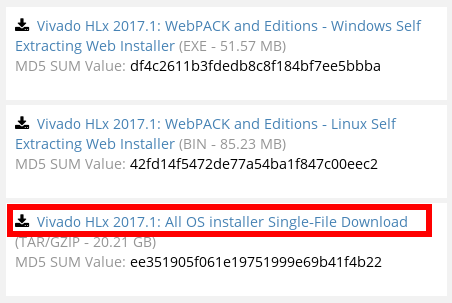
\includegraphics[scale=0.6]{figures/xilinx_vivado_2017_download}}
	\caption{Xilinx Vivado 2017.1 Download}
\end{figure}
\item If installing Xilinx tools in a permission-restricted directory, you may need to change the umask temporarily:\newline
\code{\% sudo su -}\newline
\code{\% umask 0002}
\item Extract the tarball:\newline
\code{\% tar -xf Xilinx\_Vivado\_SDK\_2017.1\_0415\_1.tar.gz}
\item Enter the resulting directory and run the installer:\newline
\code{\% cd Xilinx\_Vivado\_SDK\_2017.1\_0415\_1}\newline
\code{\% ./xsetup}\newline
\pagebreak
\item Run through the installation process. Refer to the images below when applicable.
\begin{figure}[H]
	\centerline{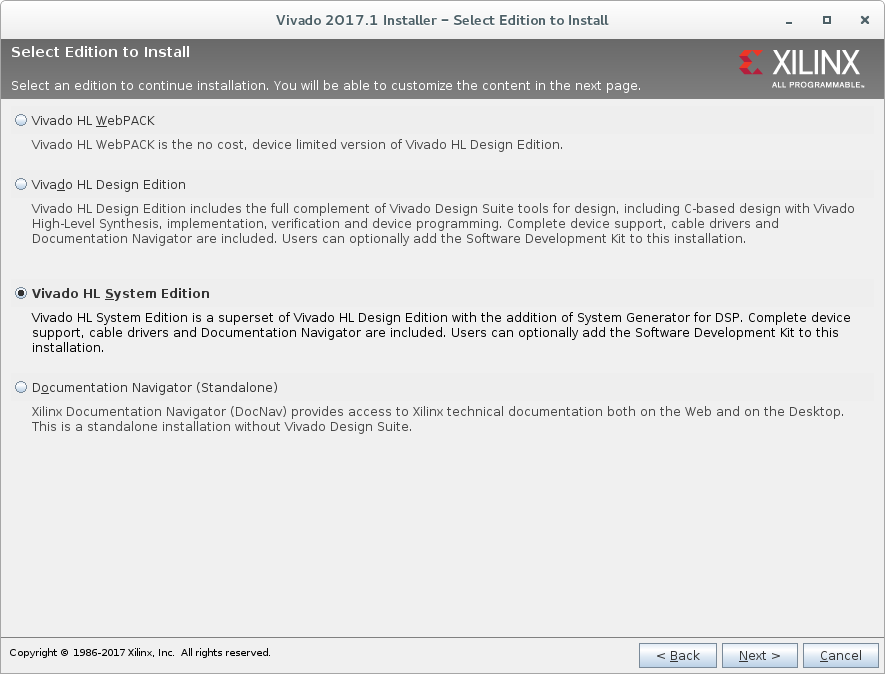
\includegraphics[scale=0.4]{figures/xilinx_vivado_2017_install}}
	\caption{Xilinx Vivado Installer}
\end{figure}
We do not direct you to acquire a license, but if you do not already have one, you will need to select ``Acquire or Manage a License Key'' in the image below.
\begin{figure}[H]
	\centerline{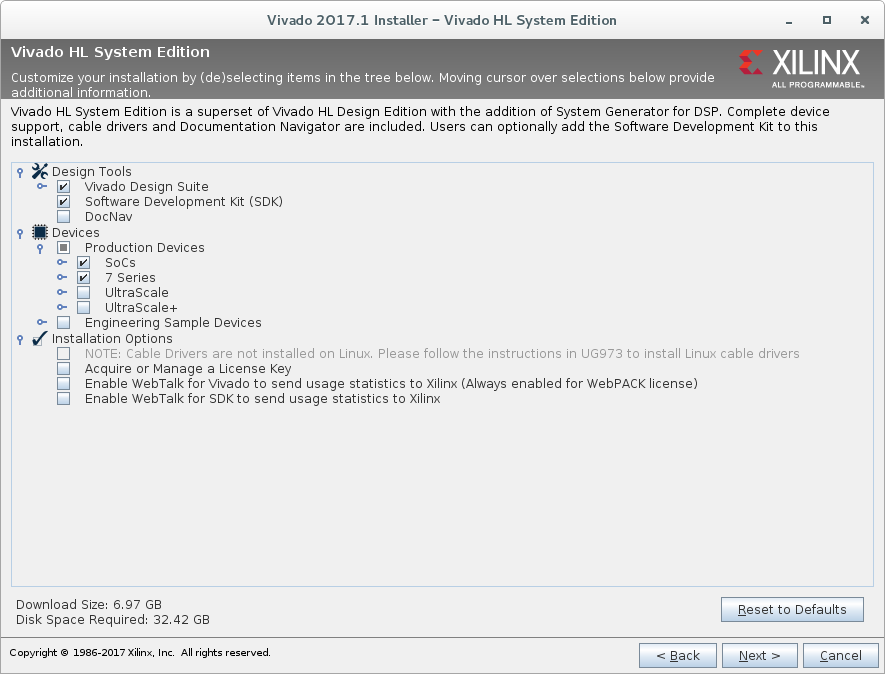
\includegraphics[scale=0.4]{figures/xilinx_vivado_2017_choose_installation}}
	\caption{Xilinx Vivado Installation Choice}
\end{figure}
\pagebreak
Take note of the installation directory chosen (e.g. \code{/opt/Xilinx}) as well as the Vivado version (e.g. \code{2017.1}) for later use.
\begin{figure}[H]
	\centerline{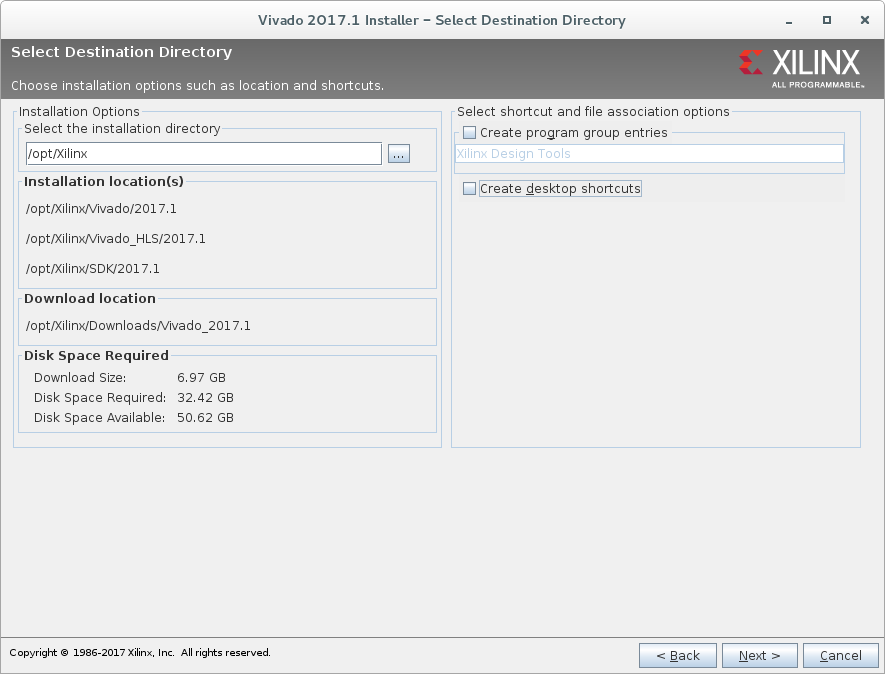
\includegraphics[scale=0.4]{figures/xilinx_vivado_2017_install_location}}
	\caption{Xilinx Vivado Install Location}
\end{figure}
\end{enumerate}
% TODO: Make this next section a snippet because it is copypasted a lot
\subsubsection{OpenCPI Considerations}
\begin{enumerate}
\item Note that sourcing the ``\verb+<Vivado-install-dir>/Vivado/<Vivado-version>/settings64.sh+'' script will interfere with OpenCPI's environment setup. Accordingly, it is recommended to always source these scripts and execute any follow-on commands in a \textit{separate terminal}.
\item To use OpenCPI with any Xilinx Vivado installation, it is required to set the following environment variables before running OpenCPI commands. Note that each of the following \code{export} statements is only necessary under the following conditions:
\begin{itemize}
\item When using a non-default installation location (i.e. anything other than \path{/opt/Xilinx})
\item When Vivado \textit{and} ISE are both being used and are installed in different locations
\item Or when multiple versions of Vivado are installed and you wish to use a version other than the newest.
\end{itemize}

\subitem \code{\% export OCPI\_XILINX\_VIVADO\_DIR=<Vivado-install-dir>}
\subitem \code{\% export OCPI\_XILINX\_VIVADO\_VERSION=<Vivado-version>}

\end{enumerate}
If OpenCPI has been installed prior to the Vivado installation, and it is desired to make the aforementioned environment variables set automatically upon login for all users, the variables should be added in \code{/opt/opencpi/cdk/env.d/xilinx.sh}. Logging out and logging back into the user account will apply said variables.
\subsubsection{Xilinx Vivado 2013.4 SDK Only Installation in CentOS~6/7}
\label{sec:viv_sdk}
\begin{enumerate}
\item Download the Vivado 2013.4 Standalone SDK installation files from Xilinx's download site:
\url{https://www.xilinx.com/support/download/index.html/content/xilinx/en/downloadNav/vivado-design-tools/archive.html}. Navigate to ``2013.4'' $\rightarrow$ ``Software Development Kit''. A Xilinx account will be required.

\begin{figure}[H]
	\centerline{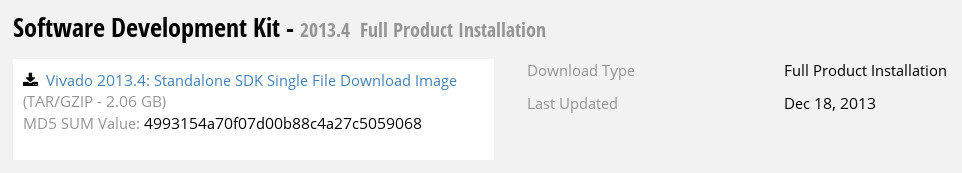
\includegraphics[scale=0.4]{figures/xilinx_vivado_sdk_download}}
	\caption{Xilinx Vivado 2013.4 SDK Download}
\end{figure}
\item If installing Xilinx tools in a permission-restricted directory, you may need to change the umask temporarily:\newline
\code{\% sudo su -}\newline
\code{\% umask 0002}
\item Extract the tarball:\newline
\code{\% tar -xf Xilinx\_SDK\_2013.4\_1210\_1.tar}
\item Enter the resulting directory and run the installer:\newline
\code{\% cd Xilinx\_SDK\_2013.4\_1210\_1}\newline
\code{\% ./xsetup}\newline
\pagebreak
\item Run through the installation process. Refer to the images below when applicable.
\begin{figure}[H]
	\centerline{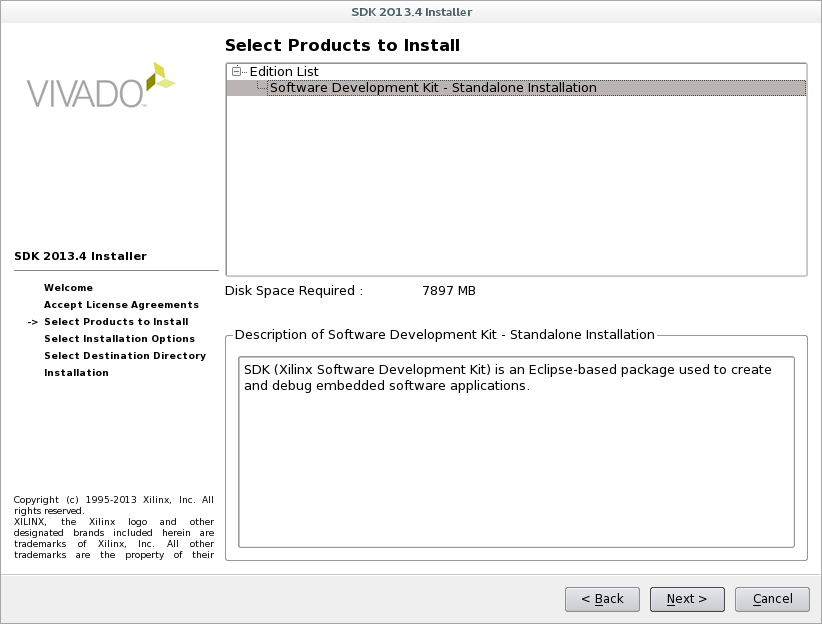
\includegraphics[scale=0.4]{figures/xilinx_vivado_sdk_install}}
	\caption{Xilinx Vivado SDK Installer}
\end{figure}

\begin{figure}[H]
	\centerline{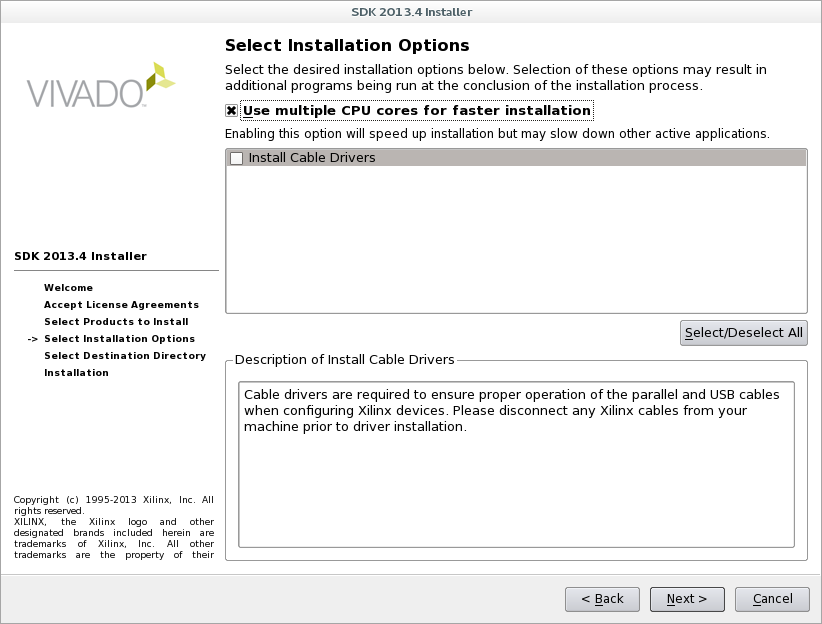
\includegraphics[scale=0.4]{figures/xilinx_vivado_sdk_choose_installation}}
	\caption{Xilinx Vivado SDK Installation Choice}
\end{figure}
\pagebreak
Take note of the installation directory chosen (e.g. \code{/opt/Xilinx}) as well as the Vivado version (e.g. \code{2013.4}) for later use.
\begin{figure}[H]
	\centerline{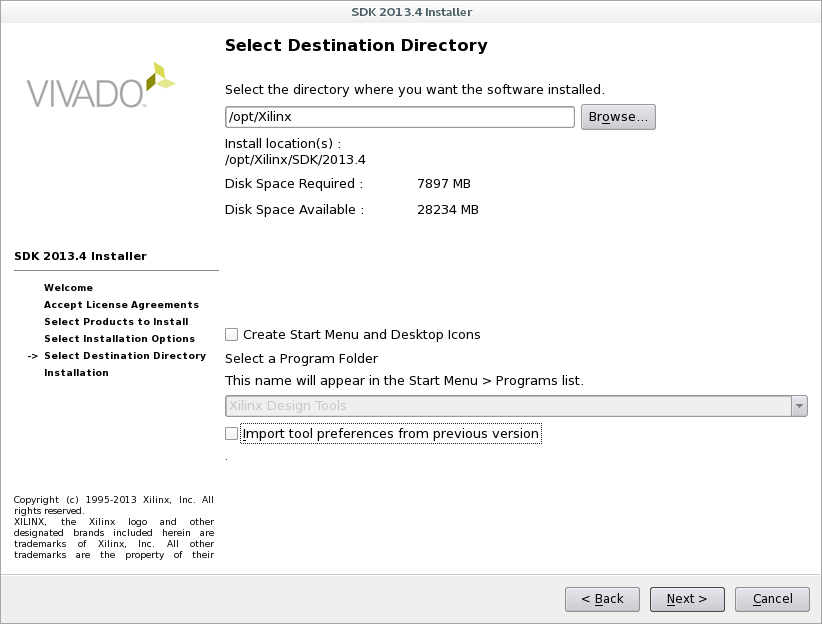
\includegraphics[scale=0.4]{figures/xilinx_vivado_sdk_install_location}}
	\caption{Xilinx Vivado SDK Install Location}
\end{figure}
\end{enumerate}
\end{flushleft}

\subsection{Xilinx ISE 14.7 Installation in CentOS~6/7}
\label{sec:ise}
\begin{flushleft}
\begin{enumerate}
\item Download the ISE 14.7 installation files from Xilinx's download site:
\url{https://www.xilinx.com/support/download/index.html/content/xilinx/en/downloadNav/design-tools.html}. A Xilinx account will be required.
\begin{figure}[ht]
	\centerline{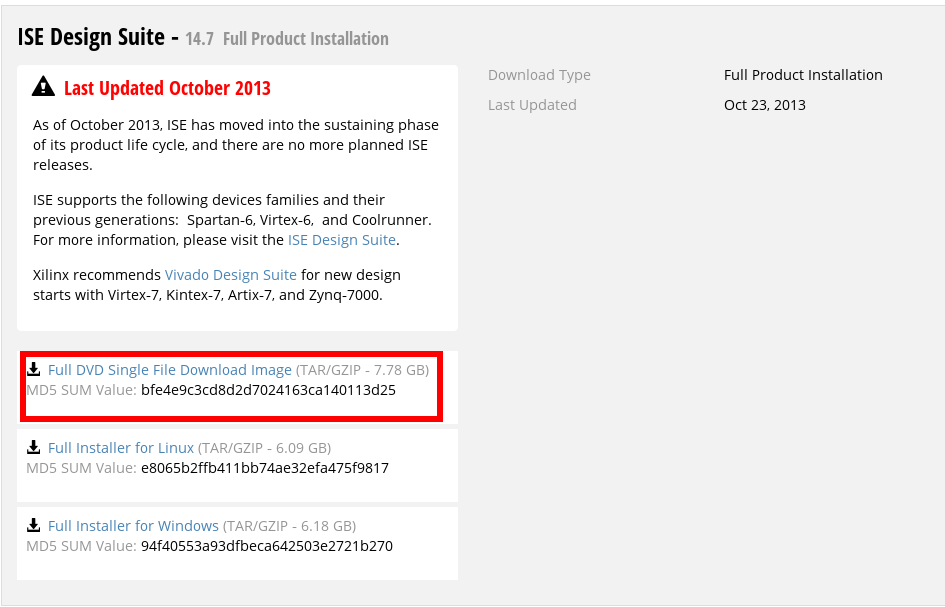
\includegraphics[scale=0.4]{figures/xilinx_ise_download}}
	\caption{Xilinx ISE Download}
\end{figure}
\item If installing Xilinx tools in a permission-restricted directory, you may need to change the umask temporarily:\newline
\code{\% sudo su -}\newline
\code{\% umask 0002}
\item Extract the tarball:\newline
\code{\% tar -xf Xilinx\_ISE\_DS\_14.7\_1015\_1.tar}
\item Enter the resulting directory and run the installer:\newline
\code{\% cd Xilinx\_ISE\_DS\_14.7\_1015\_1}\newline
\code{\% ./xsetup}\newline
\pagebreak
\item Run through the installation process. Refer to the images below when applicable. Note that the checkbox for cable drivers is left unchecked. Cable driver installation, if necessary, should be handled after this installation is complete. See section \ref{sec:cable} for more information.
\begin{figure}[H]
	\centerline{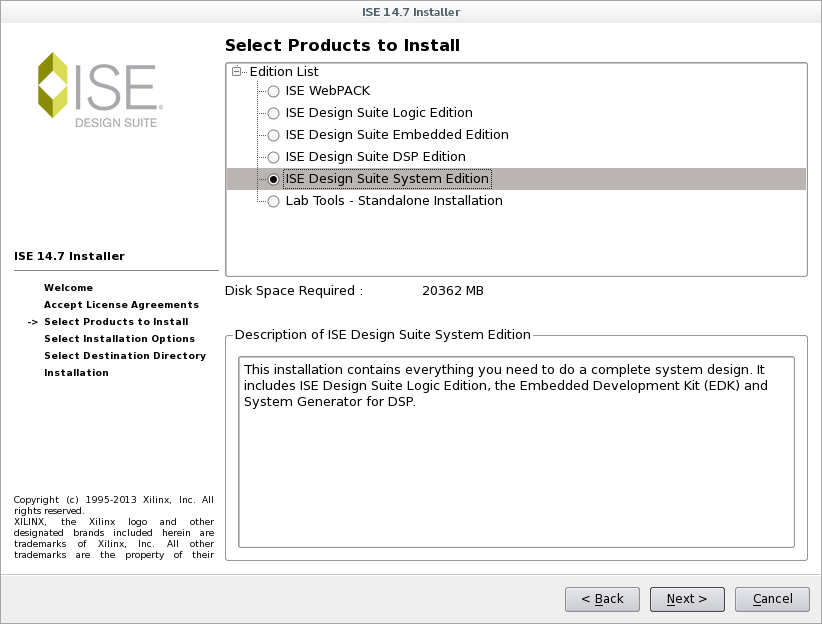
\includegraphics[scale=0.4]{figures/xilinx_ise_install}}
	\caption{Xilinx ISE Installer}
\end{figure}

\begin{figure}[H]
	\centerline{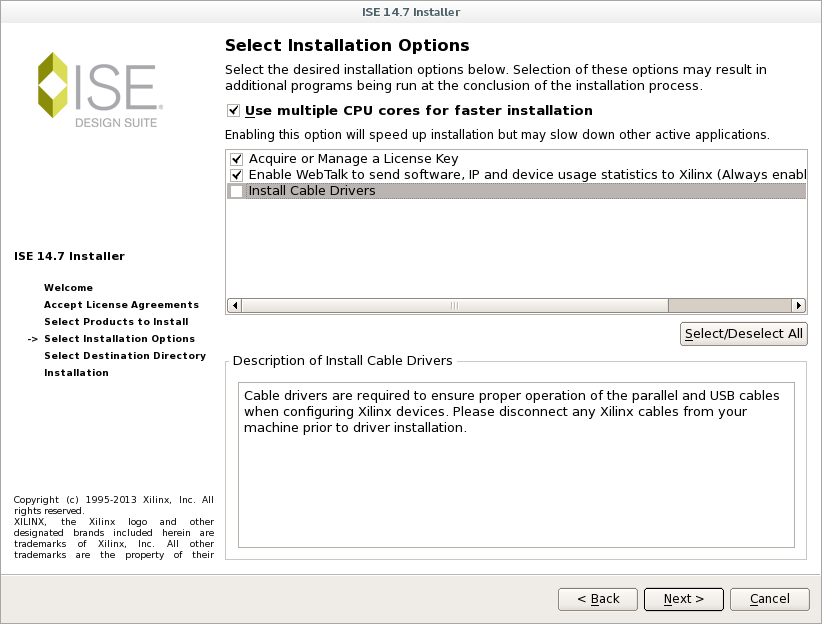
\includegraphics[scale=0.4]{figures/xilinx_labtools_choose_installation}}
	\caption{Xilinx ISE Installation Choice}
\end{figure}
\pagebreak
Take note of the installation directory chosen (e.g. \code{/opt/Xilinx}) as well as the LabTools version (e.g. \code{14.7}) for later use.
\begin{figure}[H]
	\centerline{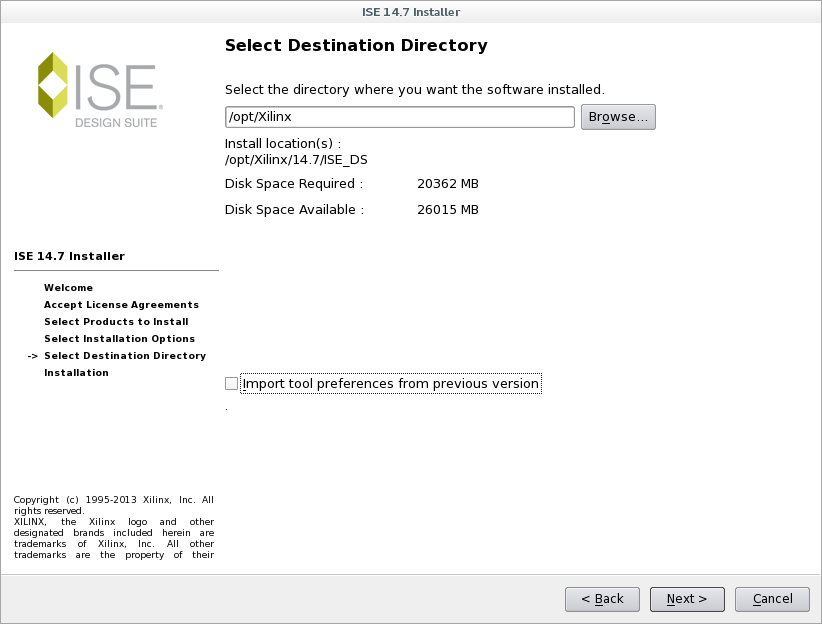
\includegraphics[scale=0.4]{figures/xilinx_ise_install_location}}
	\caption{Xilinx ISE Install Location}
\end{figure}
\end{enumerate}


\subsubsection{OpenCPI Considerations}
\label{sec:iseav}
\begin{enumerate}
\item Note that sourcing the ``\verb+<ISE-install-dir>/<version>/LabTools/settings64.sh+'' or ``\verb+<ISE-install-dir>/<version>/LabTools/settings32.sh+'' scripts will interfere with OpenCPI's environment setup. Accordingly, it is recommended to always source these scripts and execute any follow-on commands in a \textit{separate terminal}.
\item To use OpenCPI with any Xilinx ISE or LabTools installation,  it is required to set the following environment variables before running OpenCPI commands. Note that each of the following \code{export} statements are only necessary when the non-default installation location (i.e. anything other than \path{/opt/Xilinx}) or non-default version (i.e. anything other than \path{14.7}) of the tools were used.
\subitem If only one of Xilinx ISE or Xilinx LabTools is installed,
\subsubitem \code{\% export OCPI\_XILINX\_DIR=<ISE-or-LabTools-install-dir>}
\subsubitem \code{\% export OCPI\_XILINX\_VERSION=<ISE-or-LabTools-version>}
\subitem If Xilinx LabTools and ISE are the same version and installed in the same directory,
\subsubitem \code{\% export OCPI\_XILINX\_DIR=<ISE-and-LabTools-install-dir>}
\subsubitem \code{\% export OCPI\_XILINX\_VERSION=<ISE-and-LabTools-version>}
\subitem If Xilinx LabTools and ISE are the same version and are installed in different directories,
\subsubitem \code{\% export OCPI\_XILINX\_DIR=<ISE-install-dir>}
\subsubitem \code{\% export OCPI\_XILINX\_LAB\_TOOLS\_DIR=<LabTools-install-dir>}
\subsubitem \code{\% export OCPI\_XILINX\_VERSION=<ISE-and-LabTools-version>}
\subitem If Xilinx LabTools and ISE are different versions (LabTools will be ignored),
\subsubitem \code{\% export OCPI\_XILINX\_DIR=<ISE-install-dir>}
\subsubitem \code{\% export OCPI\_XILINX\_VERSION=<ISE-version>}
\end{enumerate}

If OpenCPI has been installed prior to the ISE installation, and it is desired to make the aforementioned environment variables set automatically upon login for all users, the variables should be added in \code{/opt/opencpi/cdk/env.d/xilinx.sh}. Logging out and logging back into the user account will apply said variables.
\end{flushleft}

\subsection{Xilinx LabTools 14.7 Installation in CentOS~6/7}
\label{sec:labtools}
\begin{flushleft}
\begin{enumerate}
\item Download the LabTools 14.7 installation files from Xilinx's download site:
\url{https://www.xilinx.com/support/download/index.html/content/xilinx/en/downloadNav/design-tools.html}. A Xilinx account will be required.
\begin{figure}[H]
	\centerline{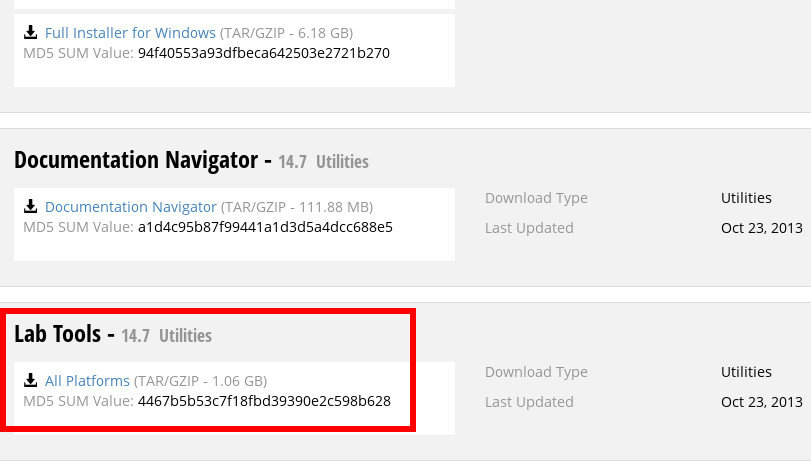
\includegraphics[scale=0.4]{figures/xilinx_labtools_download}}
	\caption{Xilinx LabTools Download}
\end{figure}
\item If installing Xilinx tools in a permission-restricted directory, you may need to change the umask temporarily:\newline
\code{\% sudo su -}\newline
\code{\% umask 0002}
\item Extract the tarball:\newline
\code{\% tar -xf Xilinx\_LabTools\_14.7\_1015\_1.tar}
\item Enter the resulting directory and run the installer:\newline
\code{\% cd Xilinx\_LabTools\_14.7\_1015\_1}\newline
\code{\% ./xsetup}\newline
\pagebreak
\item Run through the installation process. Refer to the images below when applicable. Note that the checkbox for cable drivers is left unchecked. Cable driver installation, if necessary, should be handled after this installation is complete. See section \ref{sec:cable} for more information.
\begin{figure}[H]
	\centerline{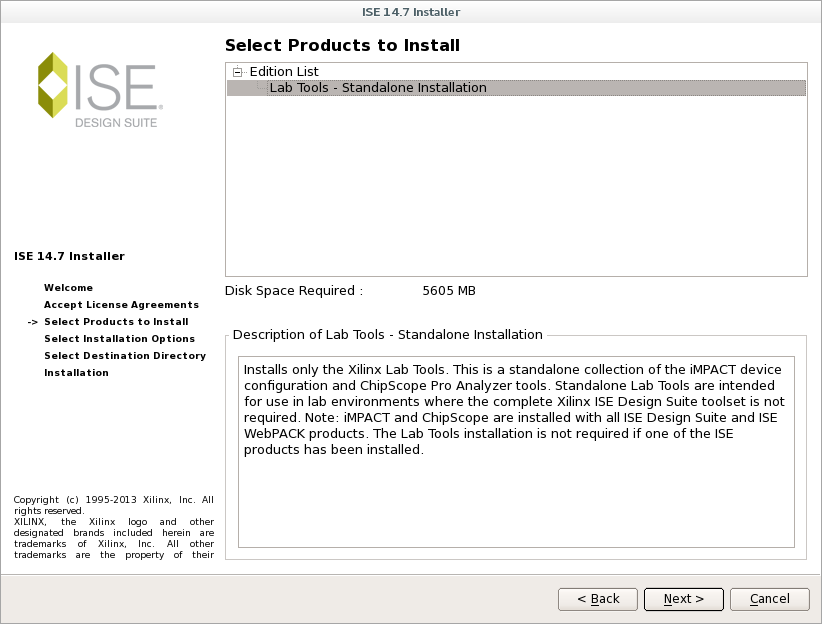
\includegraphics[scale=0.4]{figures/xilinx_labtools_install}}
	\caption{Xilinx LabTools Installer}
\end{figure}
\begin{figure}[H]
	\centerline{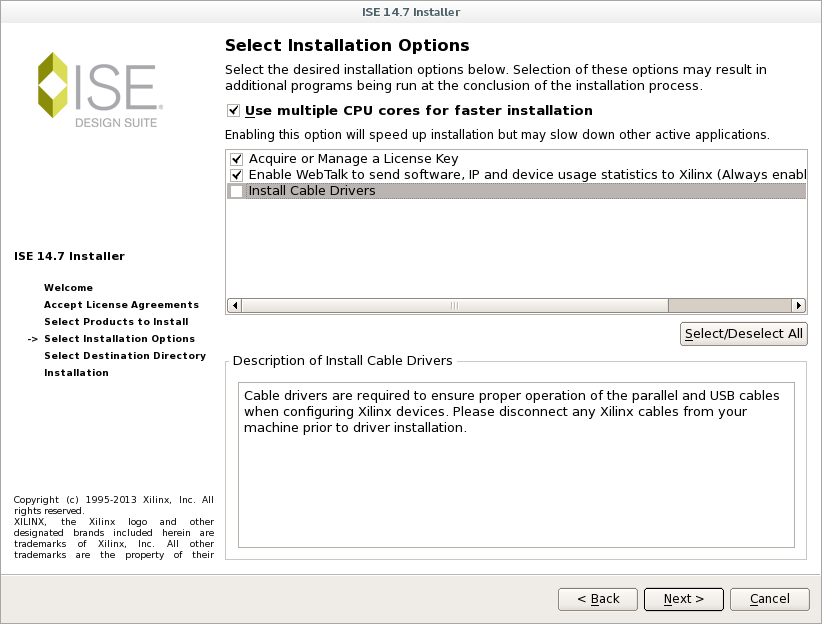
\includegraphics[scale=0.4]{figures/xilinx_labtools_choose_installation}}
	\caption{Xilinx LabTools Installation Choice}
\end{figure}
\pagebreak
Take note of the installation directory chosen (e.g. \code{/opt/Xilinx}) as well as the LabTools version (e.g. \code{14.7}) for later use.
\begin{figure}[H]
	\centerline{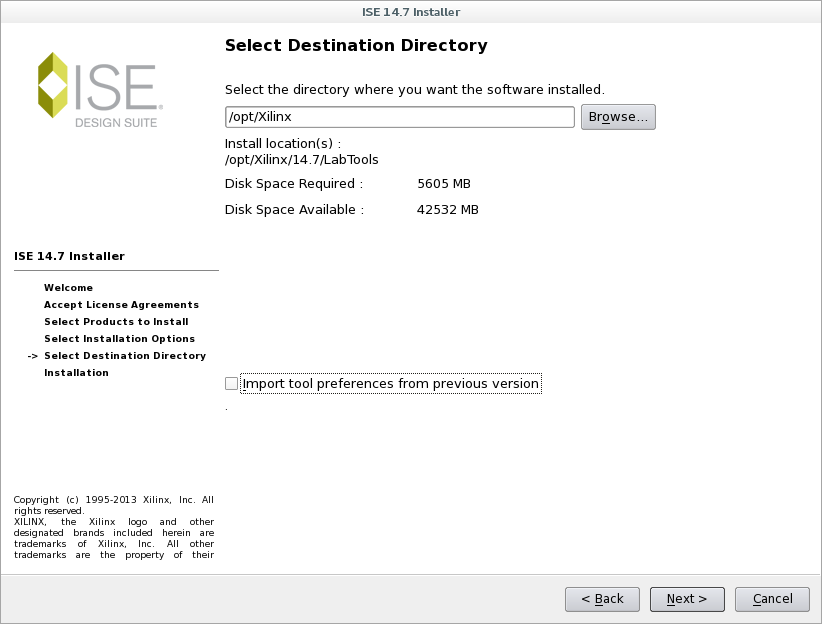
\includegraphics[scale=0.4]{figures/xilinx_labtools_install_location}}
	\caption{Xilinx LabTools Install Location}
\end{figure}
\end{enumerate}

\subsubsection{OpenCPI Considerations}
\begin{enumerate}
\item Note that sourcing the ``\verb+<LabTools-install-dir>/<version>/LabTools/settings64.sh+'' or ``\verb+<LabTools-install-dir>/<version>/LabTools/settings32.sh+'' scripts will interfere with OpenCPI's environment setup. Accordingly, it is recommended to always source these scripts and execute any follow-on commands in a \textit{separate terminal}.
\item To use OpenCPI with any Xilinx ISE or LabTools installation, it is required to set the environment variables according to Section \ref{sec:iseav} before running OpenCPI commands.
\end{enumerate}

\end{flushleft}
\pagebreak

\end{flushleft}

\subsection{Xilinx Toolset Licensing}
\label{xilinx}
A license, either WebPACK or non-WebPACK, is required for Xilinx Vivado and Xilinx ISE. Xilinx LabTools does not require a license.
\begin{enumerate}
\item The following screenshots show an ISE WebPACK license. Refer to \ref{sec:doc_overview} to determine which license is necessary. To generate a license, navigate to \url{http://www.xilinx.com/getlicense} and login (or create an account). Generate a license file:

\begin{figure}[H]
	\centerline{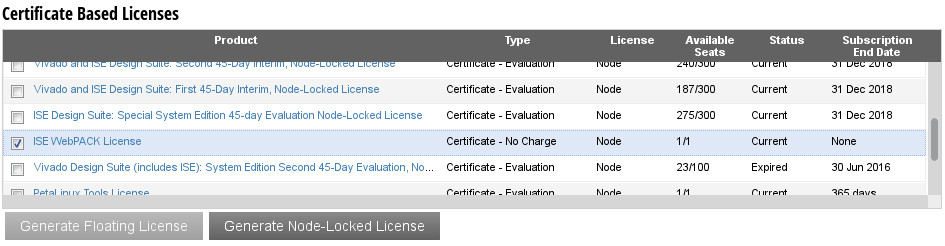
\includegraphics[scale=0.5]{./figures/xilinx_license_gen.jpg}}
	\caption{Generate Xilinx license file}
\end{figure}

\item Download the file and move it to the intended location:

\begin{figure}[H]
	\centerline{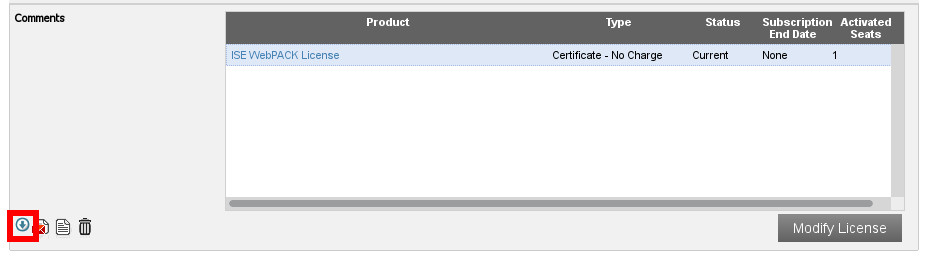
\includegraphics[scale=0.5]{./figures/xilinx_license_download.jpg}}
	\caption{Download Xilinx license file}
\end{figure}
\end{enumerate}

For use of Xilinx tools separate from OpenCPI, you will need to enable the license through the Xilinx tools.\newline

For Vivado, follow these steps:
\begin{enumerate}

\item Run ``\verb+source <Vivado-install-dir>/Vivado/<version>/settings64.sh+''.

\item Open up the license manager and load the downloaded license. The license manager can be launched either from the Vivado GUI, or from the command line by running: \\\verb+sudo <Vivado-install-dir>/Vivado/<version>/bin/vlm+\newline

Here, you can either navigate to ``Load License'' and load a copy of the license file, or you can enter the license search paths via ``Manage License Search Paths''.

\begin{figure}[H]
	\centerline{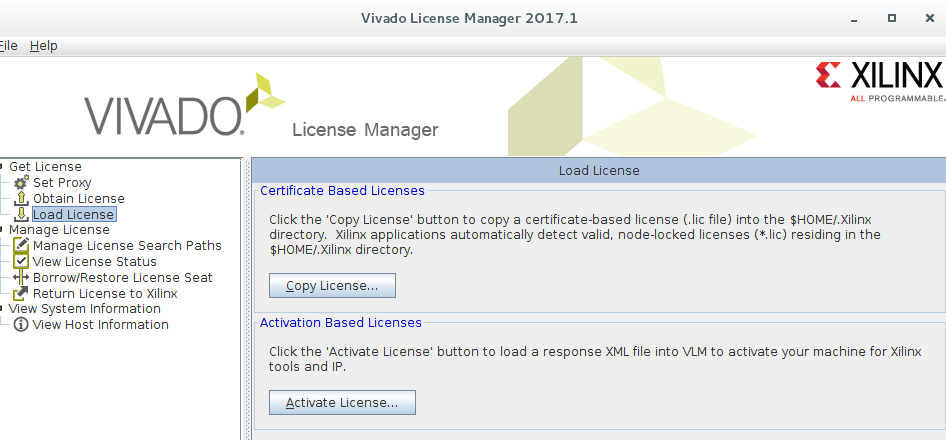
\includegraphics[scale=0.5]{./figures/xilinx_vivado_license_load}}
	\caption{Load Xilinx Vivado license file}
\end{figure}
\end{enumerate}

For ISE, follow these steps:
\begin{enumerate}
\item Run ``\verb+source <ISE-install-dir>/<version>/ISE_DS/settings64.sh+'' (or settings32.sh if the system has a 32-bit architecture).

\item Open up the license manager and load the downloaded license. The license manager can either be launched from the ISE GUI, or launched from the command line by running: \\\verb+sudo <ISE-or-LabTools-install-dir>/<version>/ISE_DS/common/bin/lin[64]/xlcm+

\begin{figure}[H]
	\centerline{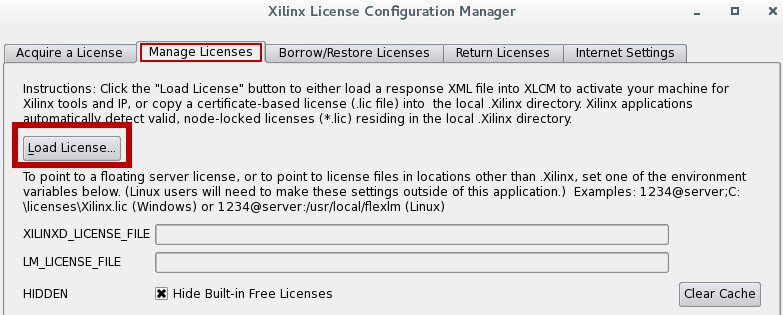
\includegraphics[scale=0.5]{./figures/xilinx_license_load.jpg}}
	\caption{Load Xilinx ISE license file}
\end{figure}
\end{enumerate}

\subsubsection{Note on node-locked licenses in CentOS~7}
If using a Xilinx node-locked license under CentOS~7, see \href{https://access.redhat.com/documentation/en-US/Red_Hat_Enterprise_Linux/7/html/Networking_Guide/sec-Disabling_Consistent_Network_Device_Naming.html}{the Red Hat Networking Guide} to revert to the
\texttt{eth\textit{N}} naming convention.

\subsubsection{OpenCPI Considerations}
\begin{enumerate}
\item Note that sourcing the ``\verb+settings64.sh+'' or ``\verb+settings32.sh+'' scripts will interfere with OpenCPI's environment setup. Accordingly, it is recommended to always source these scripts and execute any follow-on commands in a \textit{separate terminal}.
\item To enable a license for use through OpenCPI, the following is required:

	\begin{itemize}
		\item Add \verb+export OCPI_XILINX_LICENSE_FILE=<PATH_TO_LIC>+ to \verb+/opt/opencpi/cdk/env.d/xilinx.sh+. Note that this can instead point to a license server \verb+<port>@<server.ip.addr>+. If using a floating license server, it is possible to set \verb+OCPI_XILINX_LICENSE_FILE+ to the license server in addition to setting \\\verb+export XILINXD_LICENSE_FILE=<PATH_TO_LOCAL_LIC>+. This will allow use of a local license, e.g. a local WebPACK license, by default and the served floating license when WebPACK license is not sufficient.\footnote{See Xilinx ``\href{https://www.xilinx.com/support/answers/42507.html}{AR\# 42507: What are the search order and locations...}'' and ``\href{https://www.xilinx.com/support/answers/44024.html}{AR\# 44024: If a feature is licensed in multiple locations...}''}
	\end{itemize}
\end{enumerate}

\subsection{Xilinx Cable Driver Installation in CentOS~6/7}
\label{sec:cable}
\subsubsection{Vivado}
\begin{flushleft}
The steps herein are a slightly modified subset of those outlined in \url{https://www.xilinx.com/support/answers/66440.html}.
\end{flushleft}
\begin{enumerate}
\item Run the following command : \code{ls -al /etc/udev/rules.d}
\item Check if the following two files are present : \code{52-digilent-usb.rules 52-xilinx-pcusb.rules}
\item If the files above are not present, run the installer (\textit{it is important to have the JTAG cable unplugged while you perform the installation}):\\
	\code{cd <YOUR\_XILINX\_INSTALL>/data/xicom/cable\_drivers/<lin64 or lin32>/install\_script/install\_drivers;} \\
	\code{./install\_drivers;}
\end{enumerate}

\subsubsection{ISE}
\textbf{Verifying udev rules}
\begin{enumerate}
\item Run the following command : \code{ls -al /etc/udev/rules.d}
\item Check if the following file is present : \code{xusbdfwu.rules}
\item If the file is present, go to step 5. If the files above are not present, open the \code{setup\_pcusb} script and change line 26 from \code{TP\_USE\_UDEV="0"} to \code{TP\_USE\_UDEV="1"}
\item Rerun the \code{setup\_pcusb} installation script
\item \code{xusbdfwu.rules} should now be present in \code{ls -al /etc/udev/rules.d}. Open the file and change (if necessary)\newline
\code{SYSFS} to \code{ATTRS}\newline
\code{BUS} to \code{SUBSYSTEM}\newline
\code{\$TEMPNODE} to \code{\$tempnode}
\item Reload the udev rules by typing \code{udevadm control --reload-rules}
\end{enumerate}
\subsubsection{Testing Cable Driver Installation}
\textbf{ISE}
\begin{flushleft}
To verify successful cable driver installation, you can run the following:\\
\code{cd /opt/Xilinx/14.7/ISE\_DS} \\
\code{. ./settings64.sh} \\
\code{cd ~} \\
\code{echo listusbcables | impact -batch} \\
If the cable driver is successfully installed, ``\code{Using libusb.}'' will be included in the text printed to the screen.
%
%This section assumes you have completed the cable driver installation and you have OpenCPI installed.
%
%To verify successful cable driver installation, you can run the following:\newline\newline \code{/opt/opencpi/cdk/scripts/probeJtag}\newline\newline This script uses \code{impact} and enumerates the JTAG device chain. On success, it will print information such as the USB port, device serial number, and target part:
% \begin{figure}[H]
%	\centerline{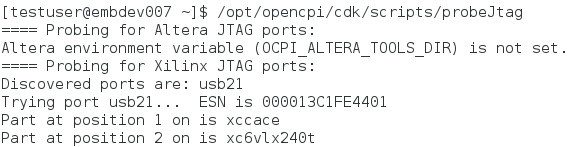
\includegraphics[scale=0.7]{./figures/probeJtag_success.jpg}}
%	\caption{Successful probeJtag}
%\end{figure}
%
%If you have an OpenCPI bitstream ready to be deployed onto your target platform, you can follow these steps to test bitstream loading:
%\begin{enumerate}
%\item Set OCPI\_PROJECT\_PATH to the project containing the platform of interest. For example, to load bitstreams to the ML605, you will need to run:\\
%\code{export OCPI\_PROJECT\_PATH=\$OCPI\_PROJECT\_PATH:<path-to-baseproject>}
%
%\item Run ``\code{ocpihdl search}'' to determine the device of interest (i.e. PCI:XXXX:XX:XX.X for PCI platforms).
%\item Load a bitstream via USB-JTAG using ocpihdl:\newline
% \code{ocpihdl load -d PCI:XXXX:XX:XX.X <path-to-bitstream>}
%\end{enumerate}
%
\end{flushleft}
\pagebreak

\newpage

\section{Intel Quartus Toolset Installation and Configuration}
\subsection{Intel Quartus Prime Standard Edition 17.1 Installation in CentOS~7}
\begin{flushleft}
\begin{enumerate}
	\item Download the Quartus Prime Standard Edition 17.1 installation files from Altera's download site: \url{https://www.intel.com/content/www/us/en/programmable/downloads/download-center.html}. Choose \verb+Standard Edition 17.1+ and either choose the ``Complete Download'', or the ``Multiple File Download'' (for this option, make sure to download the device packages of interest). An \verb+Intel Customer+ account will be required.
\item If installing Quartus tools in a permission-restricted directory, you may need to change the umask temporarily:\newline
\code{\% sudo su -}\newline
\code{\% umask 0002}
\item Extract the tarball:\newline
\code{\% tar xvf Quartus-17.1.0*.tar}
\item Run the installer:\newline
\code{\% ./setup.sh}\newline
\item Run through the installation process and choose your installation directory. Note that OpenCPI will search for Quartus Standard in \path{/opt/altera} or \path{~/intelFPGA} without any additional user settings.
\end{enumerate}

\subsubsection{OpenCPI Considerations}
It may required to set the following environment variables before running OpenCPI commands. Note that \texttt{<quartus-version>} should be replaced with the appropriate Quartus version (e.g. \code{17.1}), and \texttt{<quartus-install-dir>} should be replaced with the installation directory (\textit{e.g.} \path{~/intelFPGA}). Note also that each of the following \code{export} statements are only necessary when the non-default installation location (\textit{e.g.} anything other than \path{~/intelFPGA}, \path{/opt/intelFPGA}, \path{~/altera} or \path{/opt/Altera}), or non-default version (\textit{e.g.} anything other than the newest version) of the tools were used.\newline
\code{\% export OCPI\_ALTERA\_DIR=<quartus-install-dir>}\newline
\code{\% export OCPI\_ALTERA\_VERSION=<quartus-version>}\newline
\code{\% export OCPI\_ALTERA\_LICENSE\_FILE=<path\_to\_license\_file>}

These variables can be set automatically upon login for all users if added in \path{/opt/opencpi/cdk/env.d/altera.sh}. Logging out and logging back into the user account will apply said variables.

\end{flushleft}

\subsection{Intel Quartus Prime Pro Edition 17.0.2 Installation in CentOS~7}
\begin{flushleft}
	NOTE: Do not install Quartus Pro in the same directory as Quartus Standard because OpenCPI cannot differentiate between the two.\\
	NOTE: Quartus Pro and Quartus Standard are \textit{different tools}. The devices supported by each are different, and users should consult Intel documentation before choosing a tool edition.
\begin{enumerate}
	\item Download the Quartus Prime Pro Edition 17.0 installation files from Altera's download site: \url{https://www.intel.com/content/www/us/en/programmable/downloads/download-center.html}. Choose \verb+Pro Edition 17.0+ and either choose the ``Complete Download'', or the ``Multiple File Download'' (for this option, make sure to download the device packages of interest). An \verb+Intel Customer+ account will be required.
\item If installing Quartus tools in a permission-restricted directory, you may need to change the umask temporarily:\newline
\code{\% sudo su -}\newline
\code{\% umask 0002}
\item Extract the tarball:\newline
\code{\% tar xvf Quartus-pro-17.0.0*.tar}
\item Run the installer:\newline
\code{\% ./setup.sh}\newline
\item Run through the installation process and choose your installation directory. Note that OpenCPI will search for Quartus Pro in \path{~/intelFPGA_pro} or \path{/opt/intelFPGA_pro} without any additional user settings.
\item Download the 17.0.2 patch by navigating to the \verb+Updates+ tab and downloading ``Quartus Prime Software v17.0 Update 2''.
\item Run the installer:\newline
	\code{\% ./QuartusProSetup-17.0.2*.run}
\end{enumerate}

\subsubsection{OpenCPI Considerations}
It may be required to set the following environment variables before running OpenCPI commands. Note that \texttt{<quartus-version>} should be replaced with the appropriate Quartus version (e.g. \code{17.0} not \code{17.0.2}), and \texttt{<quartus-install-dir>} should be replaced with the installation directory (\textit{e.g.} \path{~/intelFPGA_pro}). Note also that each of the following \code{export} statements are only necessary when the non-default installation location (\textit{e.g.} anything other than \path{~/intelFPGA_pro}, \path{/opt/intelFPGA_pro}, \path{~/altera} or \path{/opt/Altera}), or non-default version (\textit{e.g.} anything other than the newest version) of the tools were used.\newline
\code{\% export OCPI\_ALTERA\_PRO\_DIR=<quartus-install-dir>}\newline
\code{\% export OCPI\_ALTERA\_PRO\_VERSION=<quartus-version>}\newline
\code{\% export OCPI\_ALTERA\_PRO\_LICENSE\_FILE=<path\_to\_license\_file>}

These variables can be set automatically upon login for all users if added in \path{/opt/opencpi/cdk/env.d/altera.sh}. Logging out and logging back into the user account will apply said variables.
\end{flushleft}

\begin{flushleft}
\subsection{Licensing Notes}
% AV-3316
If the user runs the Quartus software in its native GUI mode outside of OpenCPI, a license file configuration \textit{might} be stored in the variable \path{LICENSE_FILE} within \path{~user/.altera.quartus/quartus2.ini}; this setting overrides the \code{OCPI\_ALTERA\_LICENSE\_FILE} noted above and may cause confusion.

\end{flushleft}

\section{ModelSim Installation and Configuration}
\subsection{ModelSim DE 16.0e Installation in CentOS~7}
\begin{flushleft}
\begin{enumerate}
	\item Download the ModelSim installation files for version 10.6e.
\item If installing ModelSim tools in a permission-restricted directory, you may need to change the umask temporarily:\newline
\code{\% sudo su -}\newline
\code{\% umask 0002}
\item Run the installer:\newline
\code{\% ./install.linux64}
\item Run through the installation process and choose your installation directory. Note that OpenCPI has no default search paths for ModelSim installations.
\end{enumerate}


\subsubsection{OpenCPI Considerations}
Users will need to set the following environment variables to use ModelSim with OpenCPI. Note that \texttt{<modelsim-version>} should be replaced with the appropriate ModelSim version (e.g. \code{10.6}), and \texttt{<modelsim-install-dir>} should be replaced with the installation directory (\textit{e.g.} \path{~/modelsim_dlx}). The version variable need only be set if multiple ModelSim versions exist in this directory and the user wishes to use a version \textit{other than the most recent}.\\
\code{\% export OCPI\_MODELSIM\_DIR=<modelsim-install-dir>}\newline
\code{\% export OCPI\_MODELSIM\_VERSION=<modelsim-version>}\newline
\code{\% export OCPI\_MODELSIM\_LICENSE\_FILE=<path\_to\_license\_file>}

These variables can be set automatically upon login for all users if added in \path{/opt/opencpi/cdk/env.d/modelsim.sh}. Logging out and logging back into the user account will apply said variables.
\subsection{Compile Xilinx/Zynq simulation libraries for ModelSim}

	This section describes how to compile Xilinx simulation libraries of a device(s) for a particular 3rd party simulator, such as ModelSim.

	\begin{enumerate}
	 	\item Compile Xilinx libraries for ModelSim
		\item Modify \texttt{modelsim.ini} to include path of compiled Xilinx libraries
	\end{enumerate}

\subsubsection{Compile Vivado's simulation libraries}
	This section provides the steps necessary to compile Xilinx Vivado's simulation libraries of the Zynq device, for ModelSim. If using ModelSim 10.4c, note that Vivado 2017.1 does not support compilation of simulation libraries for ModelSim versions earlier than 10.5c. Therefore, if using a ModelSim 10.4c, you will need to use an earlier version of Vivado (\textit{e.g} 2015.4) to compile the simulation libraries. For this example, we use Vivado 2017.1 with ModelSim DE 10.6e.

\begin{flushleft}
	\begin{enumerate}
		\item Open a terminal window and switch the user to root:
			\subitem \code{> sudo su -}
		\item Configure the terminal for Xilinx Vivado by sourcing the setup script (for bash):
			\subitem \code{> source /opt/Xilinx/Vivado/<version>/settings64.sh}
		\item Launch Vivado:
			\subitem \code{> vivado}
		\item Select Tools $\rightarrow$ Compile Simulation Libraries...
		\item Select the following:
			\subitem Simulator: ModelSim Simulator
			\subitem Language: VHDL
			\subitem Library: All
			\subitem Family: Zynq-7000
			\subitem Compiled library location: \path{/opt/Xilinx/Vivado/<version>/vhdl/modelsim/<version>/lin64}
			\subitem Simulator executable path: \path{/opt/Modelsim/modelsim_dlx/linuxpe}
			\subitem Compile 32-bit libraries: Yes
		\item Click ``Compile''
		\item Note that 2017.1 Vivado will result in errors for ModelSim versions earlier than 10.5c. Here, we show the results for Vivado 2017.1 with ModelSim DE 10.6e, and Vivado 2015.4 with ModelSim DE 10.4c.
	\begin{figure}[H]
	\centering\captionsetup{type=figure}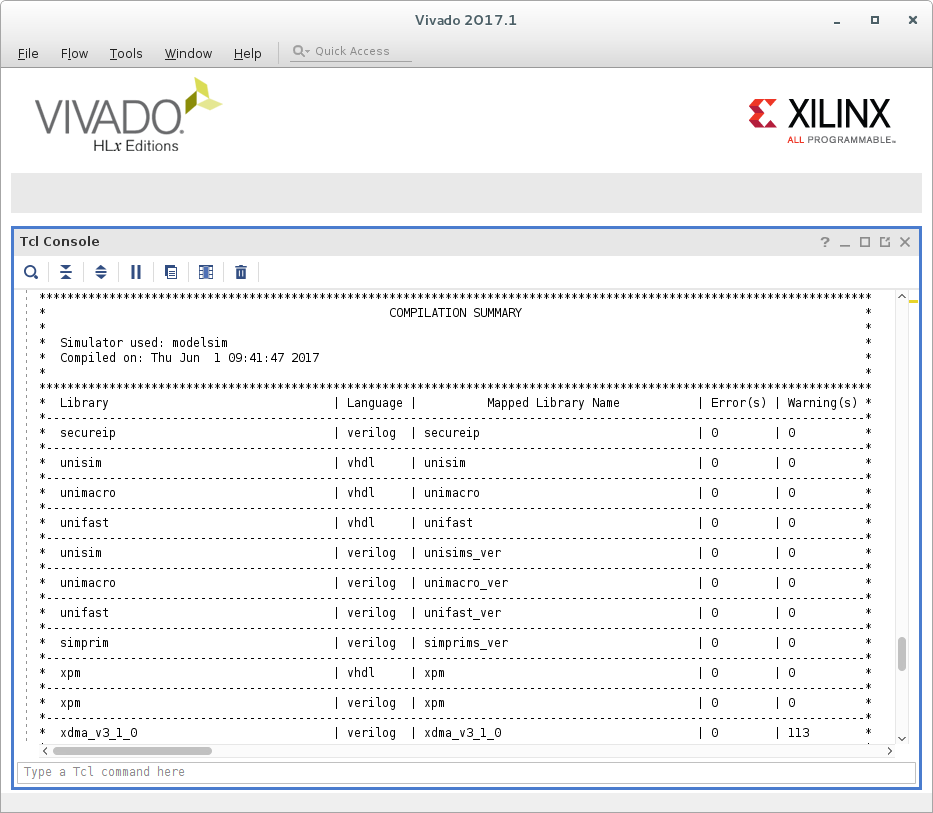
\includegraphics[scale=0.5]{figures/xilinx_vivado_2017_compsimlib_out}
		\captionof{figure}{Vivado 2017.1 Compilation Output with ModelSim DE 10.6e}
	\end{figure}
	\begin{figure}[H]
	\centering\captionsetup{type=figure}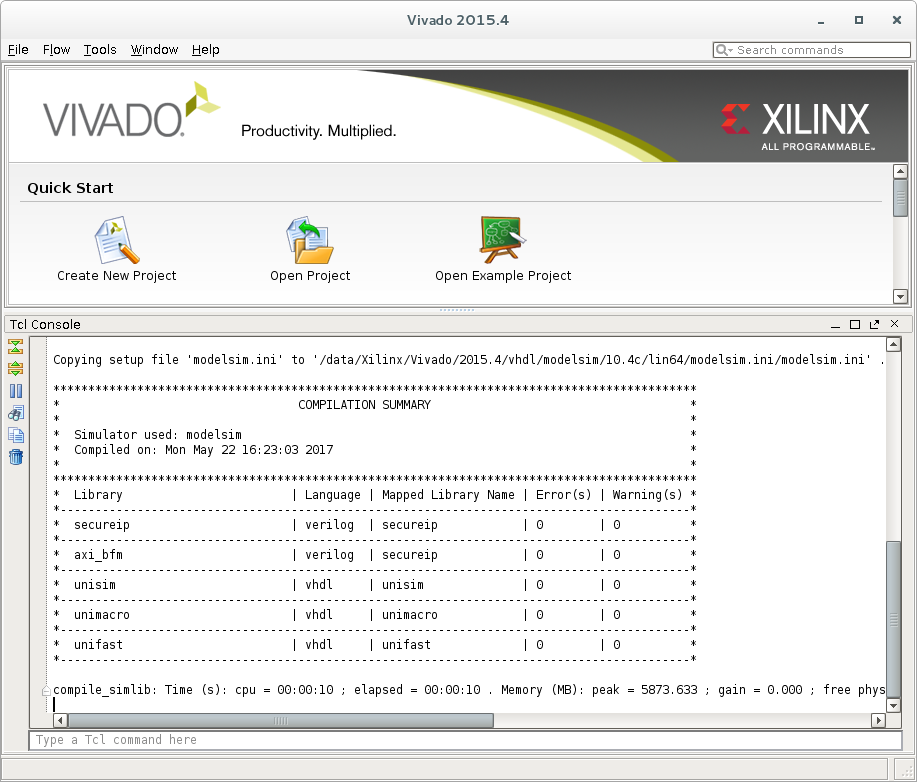
\includegraphics[scale=0.5]{figures/xilinx_vivado_2015_compsimlib_out}
		\captionof{figure}{Vivado 2015.4 Compilation Output with ModelSim DE 10.4c}
	\end{figure}
		\end{enumerate}
\end{flushleft}
\subsubsection{Compile ISE's simulation libraries}
	This section provides the steps necessary to compile Xilinx ISE's simulation libraries of the Zynq device, for ModelSim.

\begin{flushleft}
	\begin{enumerate}
	 	\item Open a terminal window and switch the user to root:
			\subitem \code{> sudo su -}
		\item Configure the terminal window for Xilinx ISE by sourcing the setup script (for bash):
			\subitem \code{> cd /opt/Xilinx/14.7/ISE\_DS/}
			\subitem \code{> source settings64.sh}
		\item Launch the Xilinx CompXLib GUI:
			\subitem \code{> cd /opt/Xilinx/14.7/ISE\_DS/ISE/bin/lin64}
			\subitem \code{> ./compxlib}

	\begin{figure}[H]
	\centering\captionsetup{type=figure}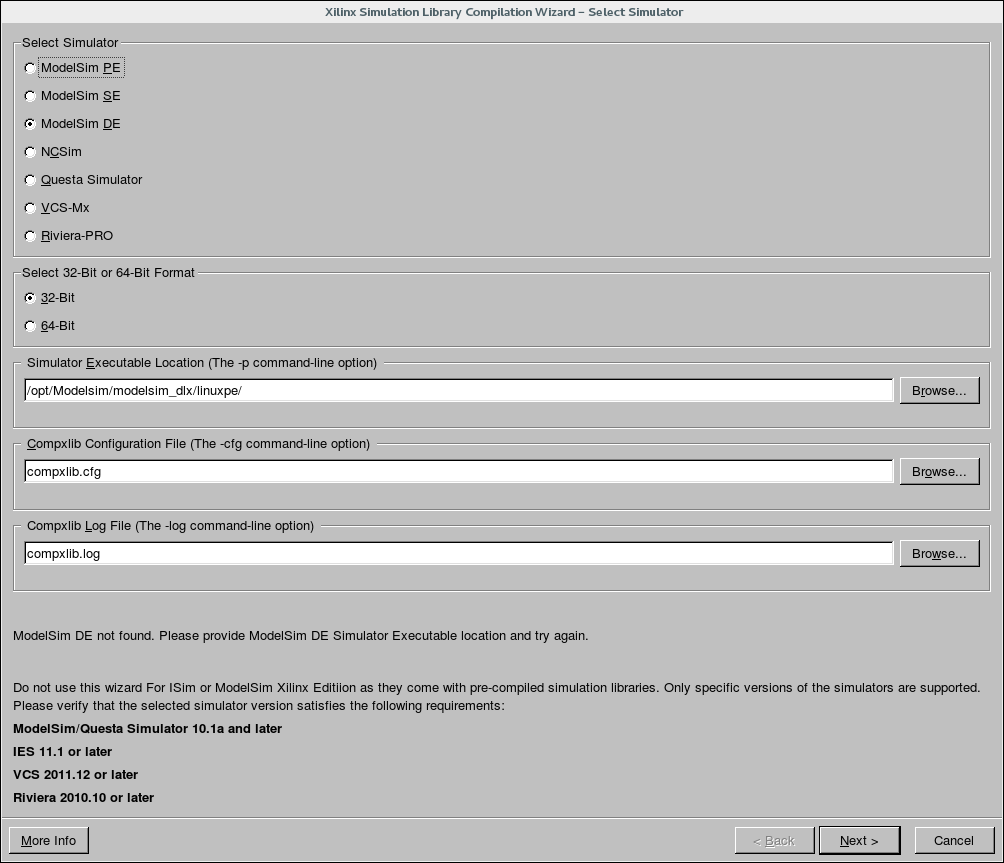
\includegraphics[scale=0.5]{figures/Xilinx_CompXLib_1_Select32bit}
		\captionof{figure}{Compilation Wizard - Select Simulator}
		\label{fig:wizard_page_1}
	\end{figure}

		\item Select ModelSim DE.
		\item Set Simulator Executable Location.
		\item Click ``Next''.

	\begin{figure}[H]
	\centering\captionsetup{type=figure}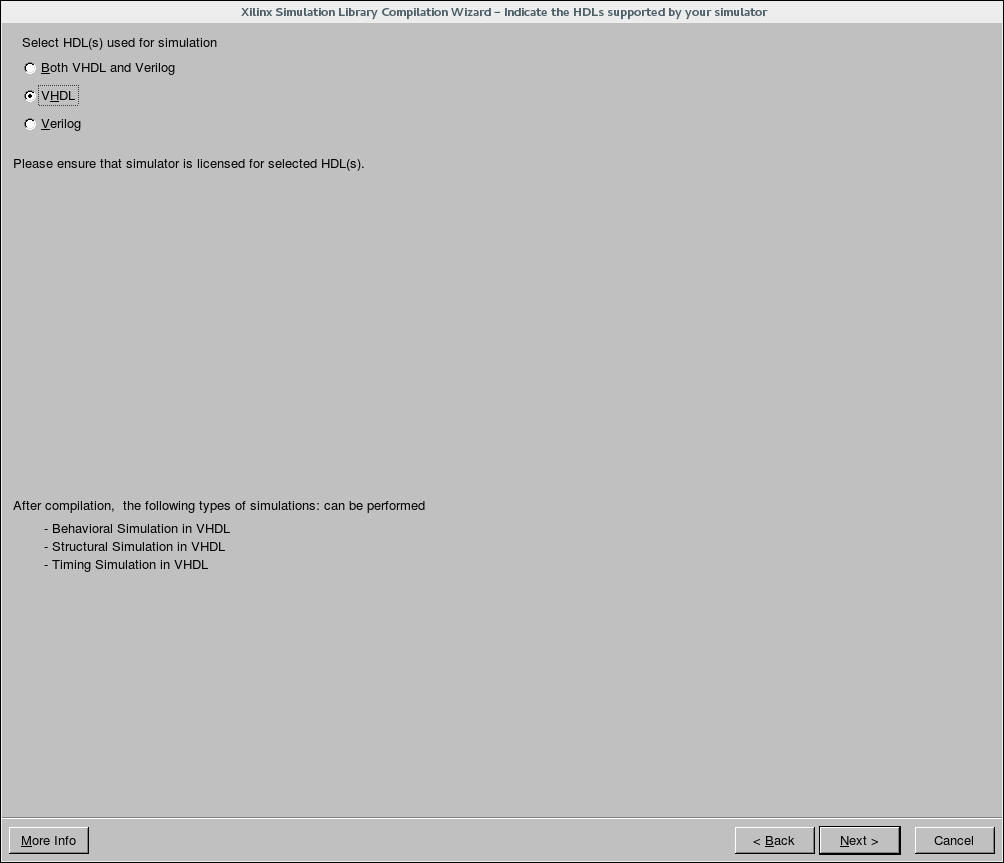
\includegraphics[scale=0.5]{figures/Xilinx_CompXLib_3_VHDLonly}
		\captionof{figure}{Compilation Wizard - HDLs to support simulator}
		\label{fig:wizard_page_3}
	\end{figure}

		\item Select ``VHDL''.
		\item Click ``Next''.

	\begin{figure}[H]
	\centering\captionsetup{type=figure}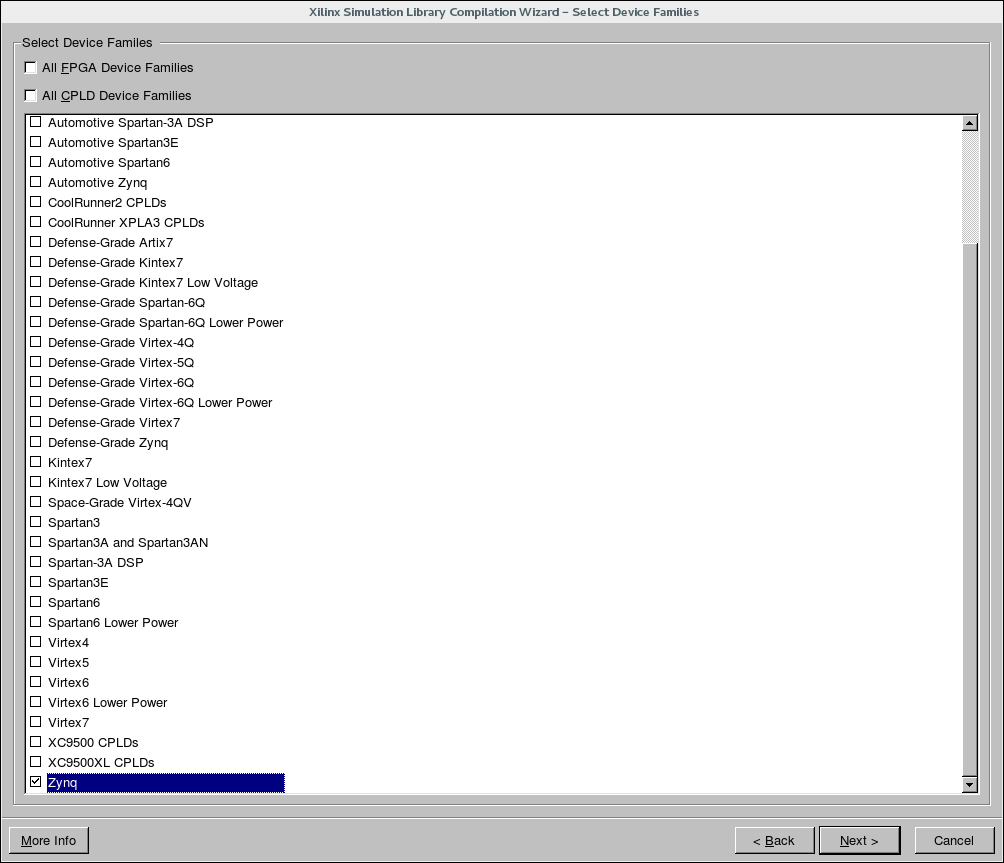
\includegraphics[scale=0.5]{figures/Xilinx_CompXLib_2_SelectZynq}
		\captionof{figure}{Compilation Wizard - Select Device Families}
		\label{fig:wizard_page_2}
	\end{figure}

		\item Uncheck ``All FPGA Device Families''.
		\item Uncheck ``All CPLD Device Families''.
		\item Check ``Zynq''.
		\item Click ``Next''.

	\begin{figure}[H]
	\centering\captionsetup{type=figure}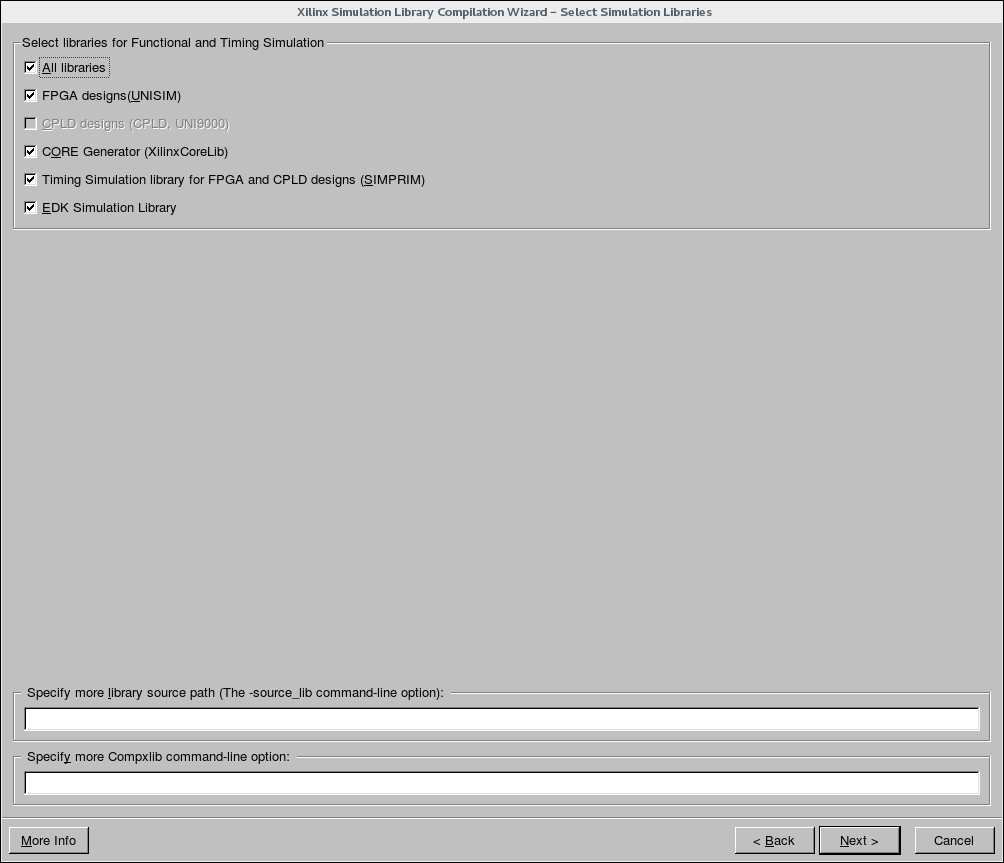
\includegraphics[scale=0.5]{figures/Xilinx_CompXLib_4_BuildAll}
		\captionof{figure}{Compilation Wizard - Select Simulation Libraries}
		\label{fig:wizard_page_4}
	\end{figure}

		\item No change.
		\item Click ``Next''.

	\begin{figure}[H]
	\centering\captionsetup{type=figure}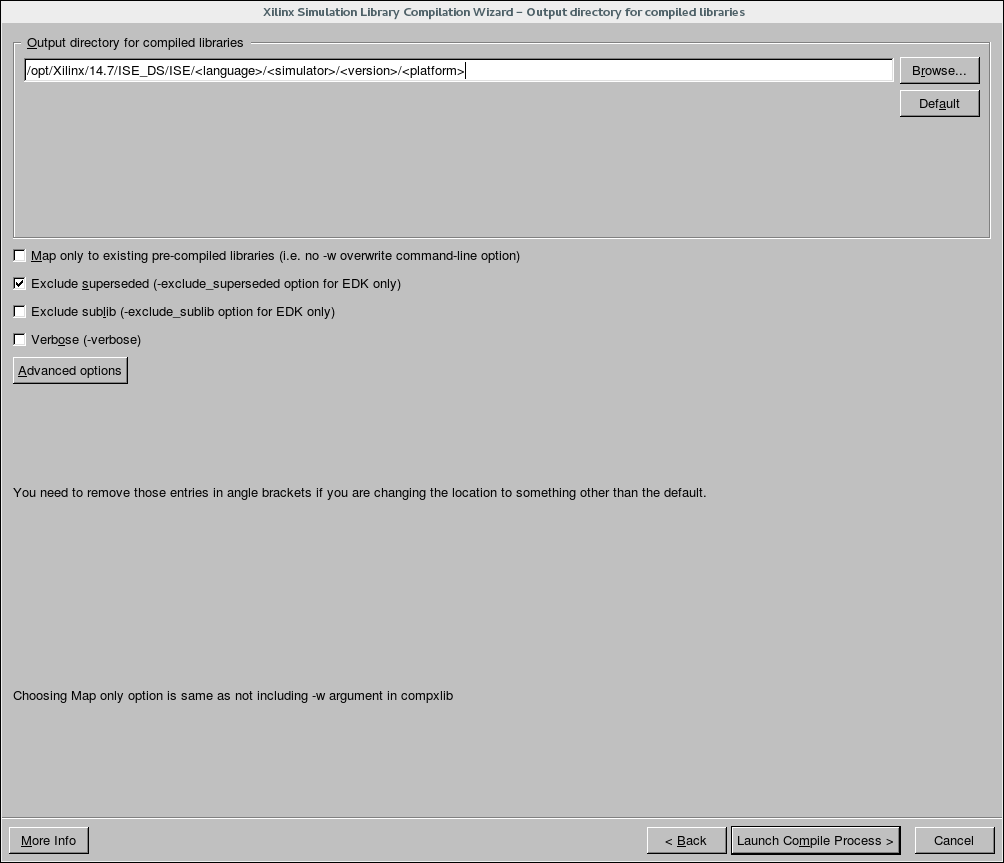
\includegraphics[scale=0.5]{figures/Xilinx_CompXLib_5_SelectDefaults}
		\captionof{figure}{Compilation Wizard - Select Output directory}
		\label{fig:wizard_page_5}
	\end{figure}

		\item Select defaults.
		\item Click ``Launch Compile Process''.
			\subitem Note: This step will take approximately 20 mins.

	\begin{figure}[H]
	\centering\captionsetup{type=figure}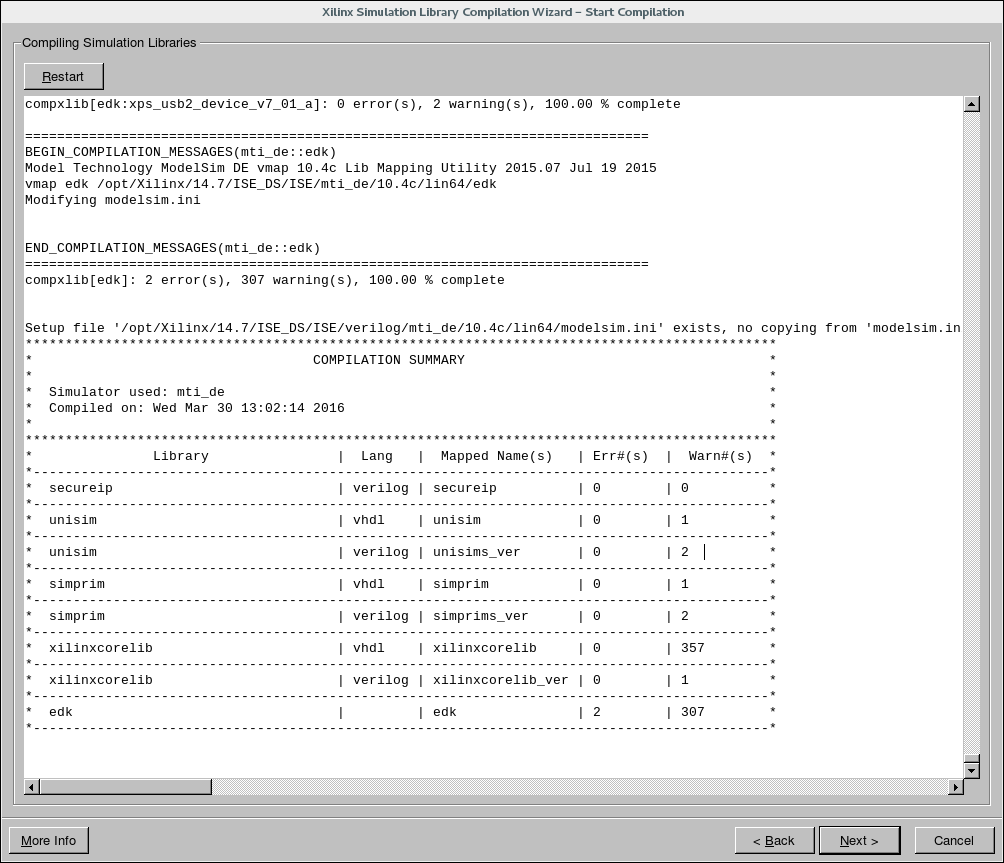
\includegraphics[scale=0.5]{figures/Xilinx_CompXLib_6_CompilationLog}
		\captionof{figure}{Compilation Wizard - Start Compilation}
		\label{fig:wizard_page_6}
	\end{figure}

		\item Click ``Next''.

	\begin{figure}[H]
	\centering\captionsetup{type=figure}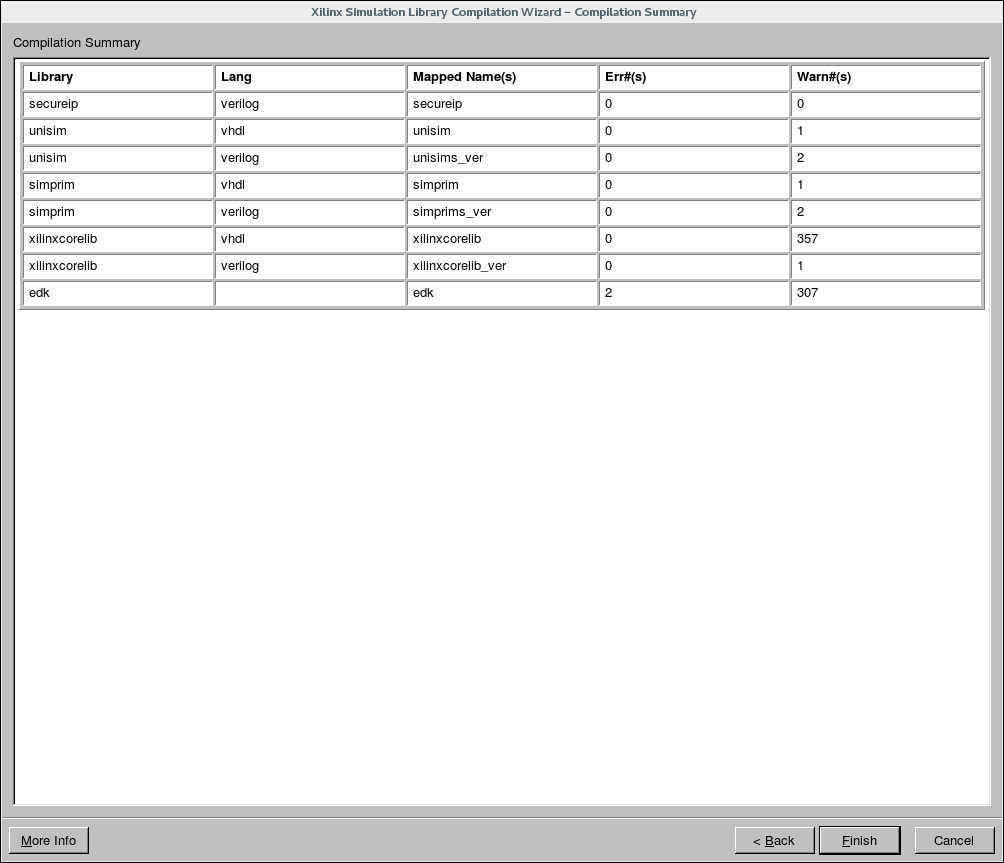
\includegraphics[scale=0.5]{figures/Xilinx_CompXLib_7_CompilationSummary}
		\captionof{figure}{Compilation Wizard - Compilation Summary}
		\label{fig:wizard_page_7}
	\end{figure}


		\item Click ``Finish''.
	\end{enumerate}

\newpage

\end{flushleft}

\subsubsection{Modify ``modelsim.ini'' to include path to built library}
	This section details the steps to modify the ``\texttt{modelsim.ini}'' file.

	\begin{enumerate}
		\item Browse to the install directory of ModelSim
			\subitem \code{> cd /opt/Modelsim/modelsim\_dlx}
		\item Open the modelsim.ini file as the root user
			\subitem \code{> vi modelsim.ini}
		\item Locate the bottom of the ``\texttt{[Library]}'' section and add the following for Vivado:
			\subitem unifast = /opt/Xilinx/Vivado/2017.1/vhdl/modelsim/10.6e/lin64/unifast
			\subitem unisim = /opt/Xilinx/Vivado/2017.1/vhdl/modelsim/10.6e/lin64/unisim
		\item Or, add the following for ISE:
			\subitem xilinxcorelib = /opt/Xilinx/14.7/ISE\_DS/ISE/vhdl/mti\_de/10.4c/lin64/xilinxcorelib
			\subitem unisim = /opt/Xilinx/14.7/ISE\_DS/ISE/vhdl/mti\_de/10.4c/lin64/unisim

	\end{enumerate}

\end{flushleft}

\end{document}
